\documentclass{article}
\usepackage[utf8]{inputenc}
\usepackage{xcolor}
\usepackage{listings}
\usepackage{minted}
\usepackage{url}
\usepackage{graphicx}
\usepackage{epstopdf}
\usepackage{caption}
\captionsetup[figure]{font=footnotesize}

\begin{document}
\title{Learning-based semantic reconstruction in binary code}
\date{}
\maketitle

\abstract{In spite of significant advances in the field of binary program analysis over the last decade, the low-level of semantics present in binary code keeps challenging the accuracy and scalability of state-of-the-art models. Of particular interest is the problem of recovering accurate data-flow information from binary code, which is key to many security applications, but unfortunately remains a bottleneck in the context of many applications. The large semantic gap between high-level representations exhibited in source-code, and low-level binary code make it a challenge to apply well-known code analysis techniques, such as those used by compilers. 
	In this project, we aim to bridge the large semantic gap between source-level and binary-level representations by combining state-of-the-art binary program analysis techniques augmented with machine learning. Our primary focus is to improve the accuracy and scalability of data-flow analysis on binary code by reconstructing type semantics.
}

\section{Introduction and definitions}
The code executed by CPUs is expressed in binary form, whereas the code written by humans is mostly written in higher-level languages such as C or C++. A so-called ``executable'' program (\textit{e.g.,} exe on Windows, ELF on Linux and other UNIXes) is in binary form, and therefore qualifies as \emph{binary program}. Source code written by humans is translated into binary by a compiler (\textit{e.g.,} CLANG). Sometimes, expert humans write code in assembly language, a representation which is much closer to binary (or ``machine'') code. The process of transforming assembly code into binary code is done by an \emph{assembler}. The inverse process, \textit{i.e.,} going from binary to assembly is called \emph{disassembly}. The latter can also be applied to binaries that have been compiled from source. Disassembly is an essential process in reverse engineering, and is generally the first step in binary program analysis. However, because of discrepancies between processor architectures, there exists many different assembly languages (\textit{e.g.,} ARM, MIPS, X86, etc\ldots). While some binary analysis frameworks only support specific architectures, most  recent models and implementations \emph{lift} binary code into an architecture-agnostic representation called \emph{Intermediate Representation (IR)}.
Figure~\ref{fig:compilation} illustrates, from a high level, the processes of compilation (with CLANG) and reverse engineering (with angr). When compiling source-code, compilers generally employ an IR which allows them to perform most program analysis tasks in a generic way, regardless of the target architecture. Similarly, modern binary analysis platforms will lift binary code into an IR in order to abstract models and techniques away from the specificities of a single CPU architecture.

\subsection{Differences between IRs}
There exists, however, a key difference between the IR produced by a compiler and the IR produced by a disassembler: the compiler extracts meta-information from source code, such as types, variables and function names, which are kept in the intermediate stages of compilation. As a result, IRs used in compilers embed such meta-information, and only discard it in the final binary (executable) program representation.
Conversely, the IR produced by disassemblers is poor, and only reflects the information present in binary.

Remember that the first step in binary program analysis is generally to \emph{disassemble} binary code. Remaining analysis stages are generally performed at the IR level. Therefore, when we speak about binary analysis, we generally speak about the process of analyzing the lifted IR instead of directly analyzing the binary code. While this is conceptually equivalent, it is syntactically different.

Because of the large semantic gap between ``poor'' IR extracted from binary and the actual original source-code of a program, it is extremely difficult to recover the latter from the former (as indicated in red in Figure~\ref{fig:compilation}).


	\begin{figure}[h]
		\centering
		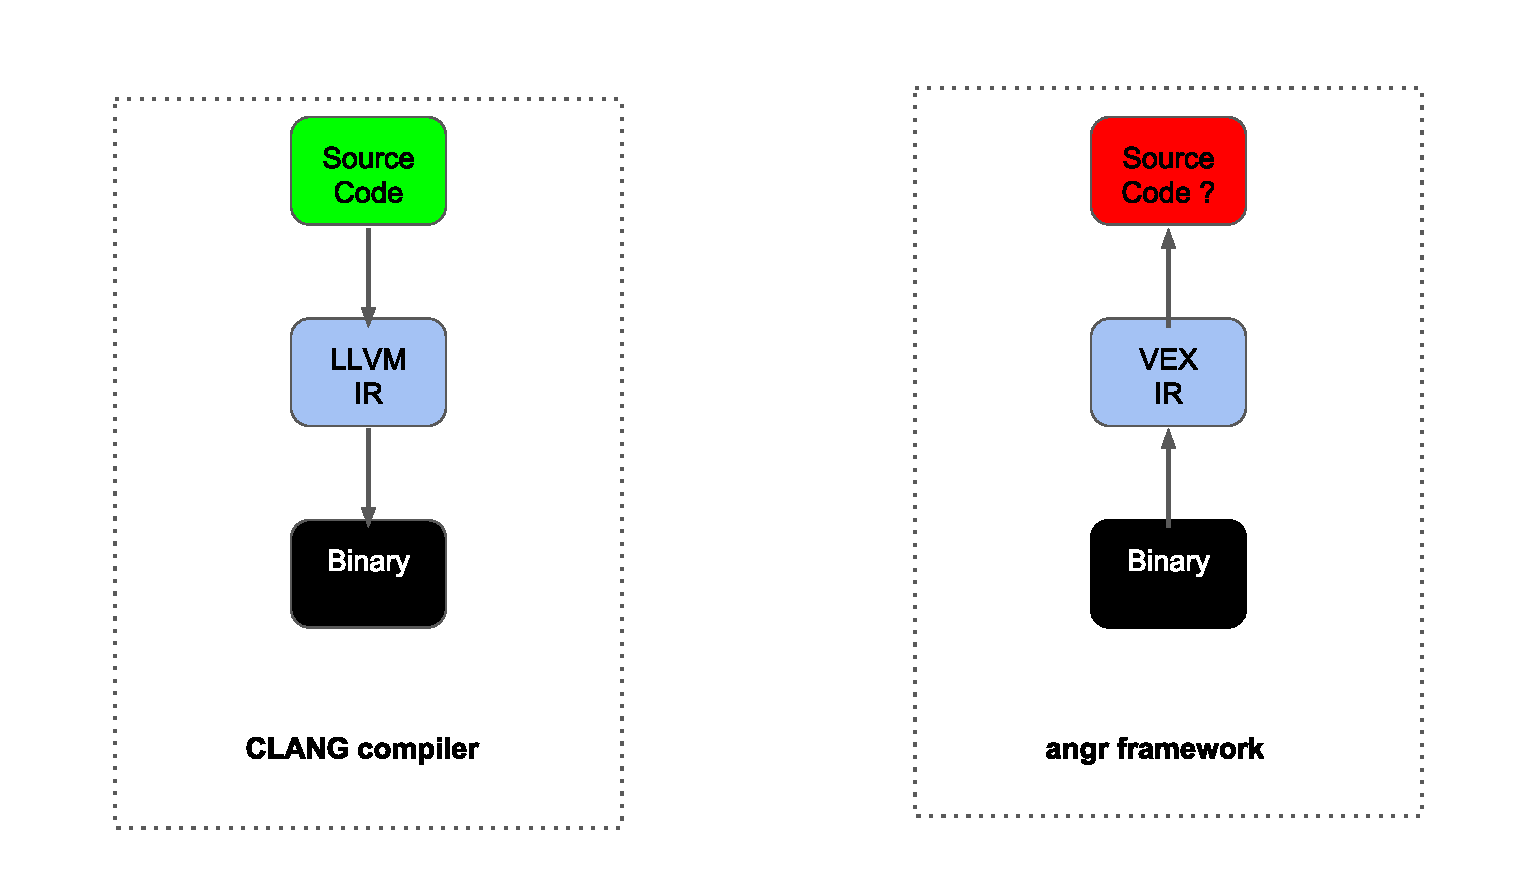
\includegraphics[width=.9\textwidth]{compilation.eps}
		\caption{Compilation with CLANG and binary analysis with angr. angr is a binary analysis platform built on top of the VEX intermediate representation.}
		\label{fig:compilation}
	\end{figure}
\end{document}

\subsection{Debug symbols}
Debugging is the process of identifying and removing errors from programs. In order for humans to relate low-level artifacts of a program (such as memory locations and registers) to high-level artifacts such as variables, functions and their associated names from the source code, it is possible to compile programs with so-called \emph{debug symbols}. These effectively provide a mapping between these representations, which greatly eases the process of manually debugging programs.
The process of removing all debug information from a binary is called \emph{stripping}, and it is done by default when distributing software (which both saves space and makes reverse-engineering difficult).

\subsection{BLAH}
